\documentclass[border=8pt]{standalone}
\usepackage[utf8]{inputenc}
\usepackage{tikz}
\usetikzlibrary{positioning}

\tikzset{
  debole/.style = {rectangle, draw, thick, fill=blue!8, double, double distance=1.5pt, minimum width=34mm, minimum height=16mm, font=\small},
  attr/.style   = {circle, draw, thick, fill=white, minimum size=5pt, inner sep=0},
  pk/.style     = {circle, draw, thick, fill=black, minimum size=5pt, inner sep=0},
  link/.style   = {thick},
  et/.style     = {font=\footnotesize}
}

\begin{document}
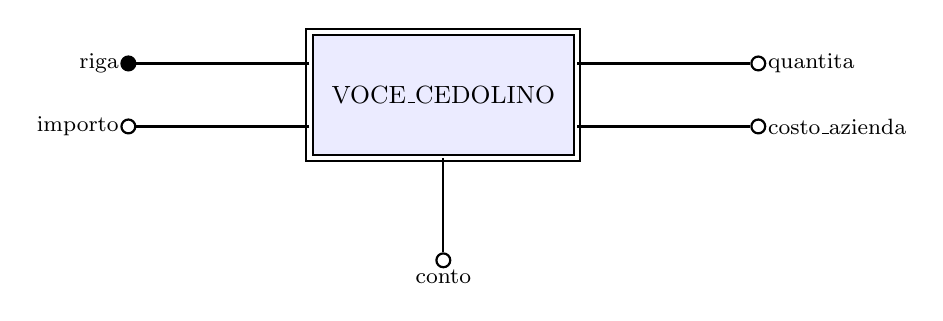
\begin{tikzpicture}
  \node[debole] (E) {VOCE\_CEDOLINO};

  \node[pk]   (r)  at (-4.0, 0.4){}; \draw[link] (-1.7, 0.4)--(r);  \node[et,left] at (r)  {riga};
  \node[attr] (im) at (-4.0,-0.4){}; \draw[link] (-1.7,-0.4)--(im); \node[et,left] at (im) {importo};

  \node[attr] (q)  at (4.0, 0.4){}; \draw[link] (1.7, 0.4)--(q);  \node[et,right] at (q)  {quantita};
  \node[attr] (ca) at (4.0,-0.4){}; \draw[link] (1.7,-0.4)--(ca); \node[et,right] at (ca) {costo\_azienda};

  \node[attr] (co) at (0,-2.1){}; \draw[link] (0,-0.8)--(co); \node[et,below] at (co) {conto};
\end{tikzpicture}
\end{document}
